\chapter{System Architecture and Design}

\section*{Introduction}
This chapter translates the requirements of Chapter~2 into a technical design. It presents the
architectural style retained, the layered organisation of the application, the cross-cutting design
decisions that structure every module, the domain model, and the relational schema that supports
it. These choices are made once here and are then applied uniformly by the ten sprints of
Chapters~4 to~7.

\section{Architectural Style}

\subsection{A Three-Tier Modular Monolith}
The platform follows a classical \textbf{three-tier} organisation (presentation, application,
data), deployed as a \textbf{modular monolith}: a single deployable artefact whose code is
partitioned into independent functional modules.

This choice deserves justification, since a microservice architecture is often the default
expectation for a management platform. Three arguments led to the monolith:

\begin{itemize}
  \item \textbf{Transactional consistency.} The PMS domain is strongly coupled: computing an
        indicator reads workload, billing, cost rates and the internal quote at once. Keeping these
        aggregates in a single transactional boundary avoids distributed transactions for no
        functional gain.
  \item \textbf{Deployment scale.} The platform targets the internal use of one company. The
        operational cost of a distributed architecture would not be repaid by the load.
  \item \textbf{Reversibility.} Partitioning the code into modules with explicit boundaries
        preserves the option of extracting a module into a separate service later, should the need
        arise.
\end{itemize}

Figure~\ref{fig:pkg} shows the ten functional packages and their dependencies.

\begin{figure}[H]
  \centering
  
\includegraphics[width=0.85\columnwidth]{img/package_diagram.png}
  \caption{Functional modules and their main dependencies}
  \label{fig:pkg}
\end{figure}

The dependency graph is deliberately acyclic and converges towards the \texttt{kpi} module, which
consumes the others without being consumed by any: the indicator engine is the end of the chain,
never a prerequisite.

\subsection{Layered Organisation}
Each module exposes the same internal layering:

\begin{itemize}
  \item \textbf{Controller} --- REST entry point, request validation, authorization annotation.
  \item \textbf{Service} --- business logic, transaction boundary, rule enforcement.
  \item \textbf{Repository} --- persistence access, implicit filtering of logically deleted rows.
  \item \textbf{Domain} --- entities and enumerations carrying the business invariants.
\end{itemize}

Conversions between entities and data transfer objects are handled by generated mappers, so that
persistence structures are never exposed directly by the API.

\section{Cross-Cutting Design Decisions}

\subsection{Authentication and Session Revocation}
Authentication rests on a short-lived JWT access token paired with an opaque refresh token stored
in an \texttt{HttpOnly} cookie. Revocation does not rely on a blacklist but on a version counter
carried by the token and compared on every request, which allows a session to be cut off instantly
without distributed state. The mechanism is detailed in Sprint~1.

\subsection{Dynamic Authorization}
The ``Role $\rightarrow$ Permission $\rightarrow$ Module'' model presented in
Section~\ref{sec:rbac} is enforced by annotating every endpoint with the permission code it
requires. No role name appears in application code. The role--permission matrix lives in the
database, which makes the authorization policy configurable data. This is the single most
structuring decision of the project and is validated in Sprint~2.

\subsection{A Hybrid Indicator Engine}
Financial indicators could be either recomputed on demand or persisted at each change. The design
retained is \textbf{hybrid}:

\begin{itemize}
  \item indicators are \textbf{recomputed on read} from live data, which guarantees that a
        dashboard never displays a stale figure;
  \item a \textbf{monthly snapshot} freezes the official state of each review, which preserves the
        history required to plot the evolution of a project.
\end{itemize}

This mirrors the reference workbook, where the dashboard reads live values while the statistics
sheet keeps one column per month. Amounts derived from the internal quote are always computed at
read time and never stored, so that no commercially sensitive value is duplicated in the database.

\subsection{Multi-Currency Handling}
Projects may be contracted in a currency different from the reporting currency. Every amount
therefore carries its currency, and conversions use a \textbf{dated rate}: each conversion applies
the rate at the business date of the amount: the invoice date for billing, the month for monthly
costs, the mission date for travel. Mission cost components are converted before summation, so that
currencies are never mixed within a total.

\subsection{Auditability and Logical Deletion}
Every business table carries creation and modification metadata and an \texttt{active} /
\texttt{deleted\_at} pair. No row is physically removed: a deletion is a state change. This
satisfies the auditability requirement and preserves the history on which the indicators depend.

\section{Domain Model}
Figure~\ref{fig:class-global} gives the overall map of the domain. The project is the aggregation
root: most business entities exist only within a project and are composed by it, while users,
roles, permissions and resources form an independent reference core.

\begin{figure}[H]
  \centering
  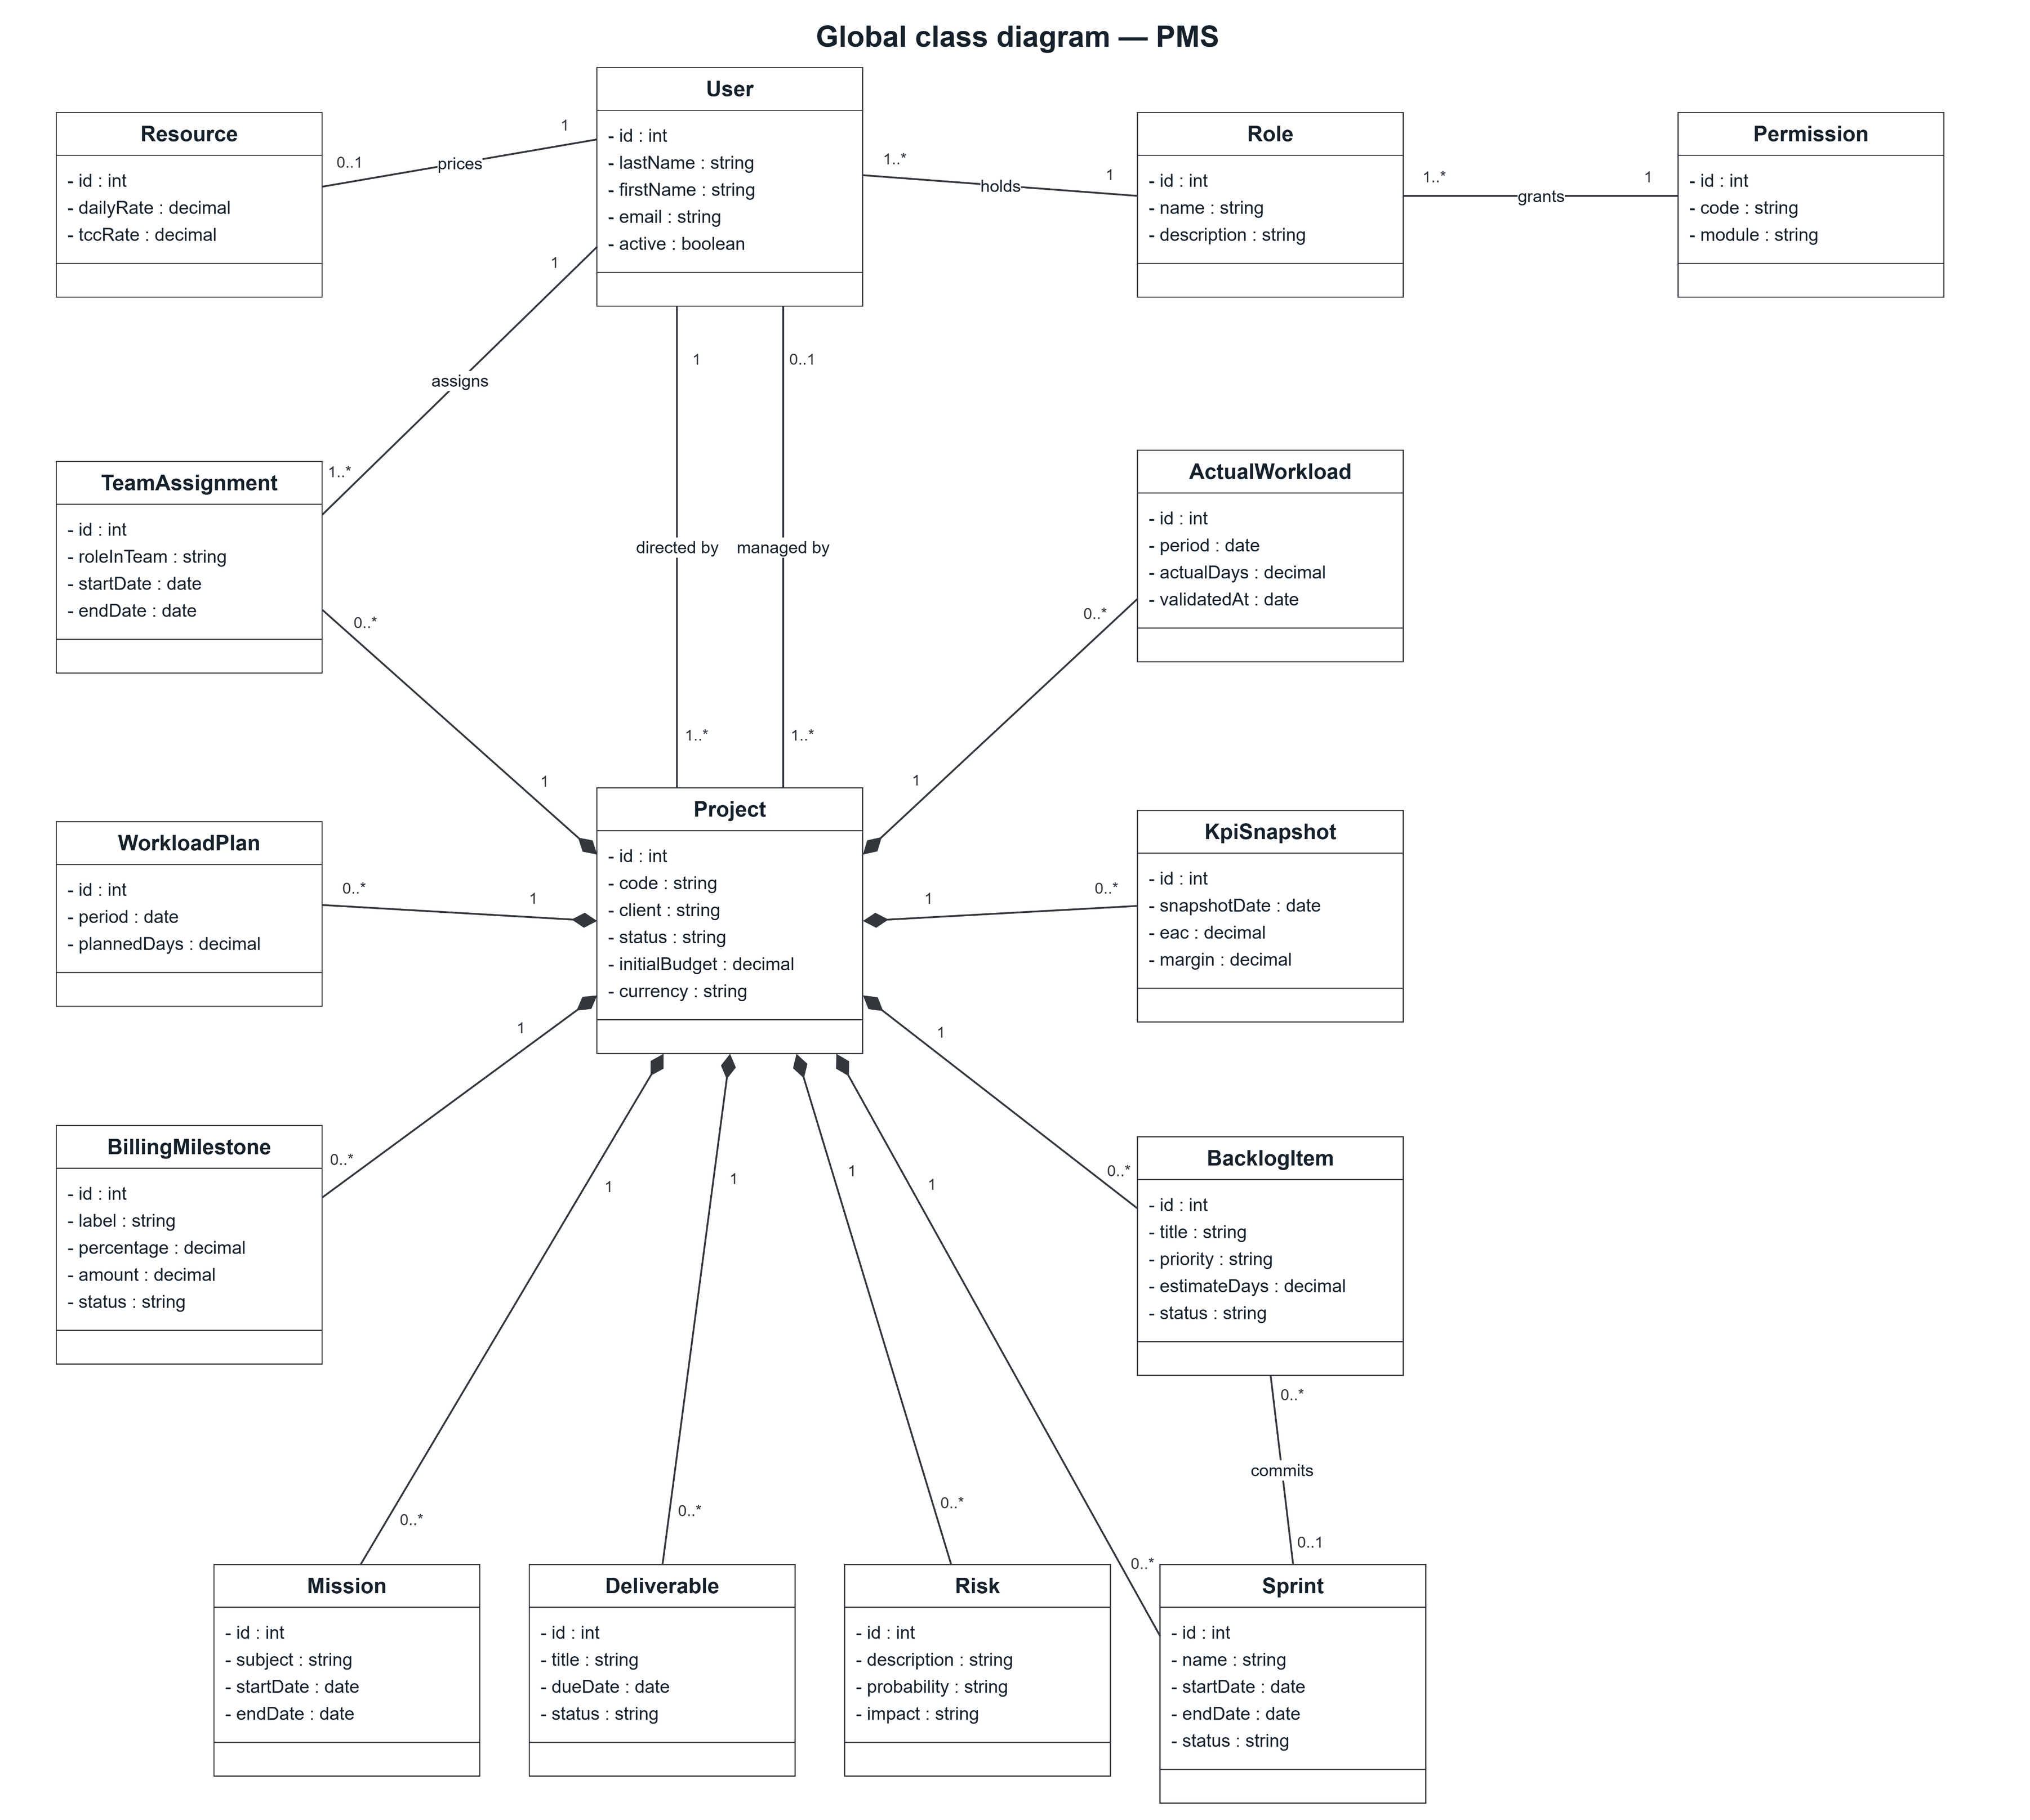
\includegraphics[width=\columnwidth]{img/class_global.png}
  \caption{Domain model --- principal classes and their associations}
  \label{fig:class-global}
\end{figure}

One reading of the diagram deserves to be made explicit, because it is easy to expect the
opposite. The four roles of the platform are not subclasses of \texttt{User}: they are rows of
the \texttt{Role} class. A user holds a role, and a role grants permissions, so the authorization
policy is data that an administrator edits rather than a hierarchy compiled into the application.
Modelling the roles as types would have contradicted that, and would have made every change of
policy a new version of the software.

The diagram stays at the level of the principal classes and their key attributes. Each sub-domain
is detailed by its own class diagram, presented in the sprint that builds it: security in
Sprint~2 (Figure~\ref{fig:class-sec}), projects and teams in Sprint~3, agile planning in
Sprint~5, financial management in Sprint~6, governance in Sprint~7, and the indicator engine in
Sprint~8.

\begin{figure}[H]
  \centering
  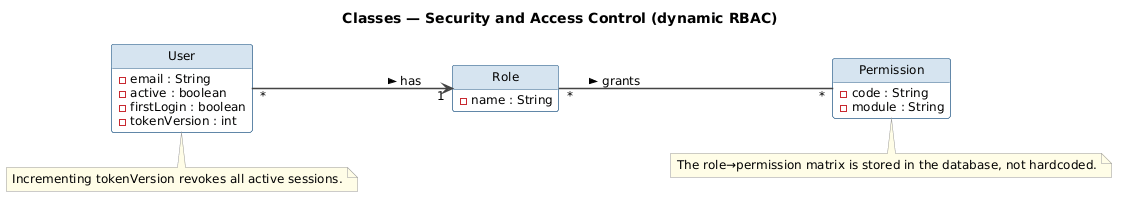
\includegraphics[width=0.75\columnwidth]{img/class_security.png}
  \caption{Class diagram --- security and access control}
  \label{fig:class-sec}
\end{figure}

\section{Database Design}

\subsection{Modelling Conventions}
The schema targets PostgreSQL and follows uniform conventions:

\begin{itemize}
  \item tables in \texttt{snake\_case}, plural; identity primary key \texttt{id};
  \item foreign keys named \texttt{<entity>\_id}; timestamps in \texttt{timestamptz};
  \item amounts stored as \texttt{numeric(18,3)} with an explicit currency column, never as
        floating point, to avoid rounding drift on financial aggregates;
  \item months stored as the \textbf{first day of the month}, making the workload a true time
        series;
  \item enumerations expressed as \texttt{varchar} constrained by \texttt{CHECK};
  \item audit columns and logical deletion on every business table.
\end{itemize}

\subsection{Logical Model}
The core of the schema is the dynamic access control: \texttt{users} references \texttt{roles}, and
\texttt{roles} relates to \texttt{permissions} through the \texttt{role\_permissions} association.
A project references its director and groups its child entities: project manager assignment (a
single active one at a time), team assignments, workload plan, actual workload, billing milestones,
missions, governance registers and KPI snapshots. A resource carries one cost rate per year and may
be linked to a user account.

\begin{longtable}{|m{3.6cm}|m{7.4cm}|m{3.4cm}|}
\hline
\textbf{Domain} & \textbf{Main tables} & \textbf{Module} \\
\hline
\endhead
\endfoot
\endlastfoot
\hline
Security / RBAC & \texttt{users}, \texttt{roles}, \texttt{permissions},
\texttt{role\_permissions} & Authentication \& RBAC \\
\hline
Reference data & \texttt{currencies}, \texttt{exchange\_rates}, \texttt{parameters}, risk scales &
Configuration \\
\hline
Resources & \texttt{resources}, \texttt{tcc} & Cost rate management \\
\hline
Projects & \texttt{projects}, \texttt{project\_manager\_assignments} & Project management \\
\hline
Teams & \texttt{team\_assignments}, \texttt{stakeholders} & Teams \\
\hline
Workload & \texttt{workload\_plan}, \texttt{actual\_workload} & Planning / Actuals \\
\hline
Billing & \texttt{billing\_milestones}, \texttt{payments}, \texttt{avenants} & Billing \\
\hline
Missions & \texttt{missions} & Mission management \\
\hline
Governance & \texttt{risks}, \texttt{deliverables}, \texttt{change\_requests}, \texttt{actions} &
Governance \\
\hline
Indicators & \texttt{kpi\_snapshots} & KPI \& Reporting \\
\hline
\caption{Catalogue of entities by domain}
\label{tab:entities}
\end{longtable}

\subsection{Monthly Time Series and Indicator Snapshots}
The Excel workbook is a resource~$\times$~month grid. Rather than reproducing twenty-five month
columns, the model is \textbf{normalised}: one row per (project, resource, month) in
\texttt{workload\_plan} and \texttt{actual\_workload}. Adding a month becomes inserting a row rather
than altering the schema.

The \texttt{kpi\_snapshots} table stores one snapshot per (project, month), which yields both the
history needed for evolution curves and fast reads for dashboards. It deliberately separates the
\textbf{labour cost} (man-days $\times$ cost rate) from \textbf{other costs} (missions and
expenses), the total aggregating the two. The original workbook blurred that distinction, which
matters when analysing why a project drifts.

\subsection{Reference Data and Migration Strategy}
A seed dataset creates the four roles, the full permission catalogue, the default role--permission
matrix, the currencies, the business parameters, the risk scales and a bootstrap administrator.

The schema is managed exclusively by \textbf{Flyway} versioned SQL migrations, with the ORM in
\texttt{validate} mode: the entities must match the schema, never generate it. The migrations
constitute the living documentation of the database and make every schema change reviewable and
reproducible.

\section{Deployment Architecture}
Figure~\ref{fig:deploy} shows the target deployment: a browser running the single-page
application, an application server exposing the REST API, and a database server. The whole
platform is a single deployable artefact, consistent with the modular monolith decision.

\begin{figure}[H]
  \centering
  
\includegraphics[width=0.55\columnwidth]{img/deployment_diagram.png}
  \caption{Deployment architecture}
  \label{fig:deploy}
\end{figure}

\section{Technical Environment}
Every technology below was chosen against the same two constraints: a single developer with eight
months, and a platform whose value lies in financial correctness rather than in scale. That
combination consistently favours mature, well-documented tools with a short path from decision to
working code, over newer ones that would have to be learned first.

\subsection{Backend}

\begin{longtable}{|m{1.9cm}|m{2.5cm}|m{10.0cm}|}
\hline
\textbf{} & \textbf{Technology} & \textbf{What it is, and why it was chosen} \\
\hline
\centering
\includegraphics[width=1.65cm,height=1.05cm,keepaspectratio]{img/logo_java.png} & Java~21 &
A statically typed, object-oriented language running on a virtual machine. Version~21 is a
long-term-support release, so the platform rests on a version that will still be maintained well
after the internship. It is also the language named by the assigned subject. \\
\hline
\centering
\includegraphics[width=1.65cm,height=1.05cm,keepaspectratio]{img/logo_springboot.png} & Spring Boot~3.3 &
A framework that turns a Java application into a self-contained, runnable server with its
dependencies already wired. It was chosen because it removes almost all configuration work:
persistence, security, validation and the REST layer are declared rather than assembled, which is
what makes ten sprints of business features possible for one developer. \\
\hline
\centering
\includegraphics[width=1.65cm,height=1.05cm,keepaspectratio]{img/logo_springsecurity.png} & Spring Security &
The security layer of the same framework, handling authentication and authorization. It was chosen
because it supports exactly the model this platform needs: a check expressed as a permission the
caller must hold, evaluated on the method rather than on the route, which is what allows the
authorization policy to live in the database instead of in the code. \\
\hline
\centering
\includegraphics[width=1.65cm,height=1.05cm,keepaspectratio]{img/logo_hibernate.png} & Hibernate (JPA) &
The object-relational mapper that translates between Java objects and database rows. It was chosen
for one property in particular: it can be told to \emph{validate} the schema at startup instead of
generating it, so a divergence between the code and the database stops the application immediately
rather than corrupting data later. \\
\hline
 & MapStruct &
A code generator that writes the conversions between entities and the objects returned by the API.
It was chosen so that persistence structures are never exposed directly by the REST layer, without
paying for that separation in hand-written boilerplate. \\
\hline
\caption{Backend technologies}
\label{tab:tech-backend}
\end{longtable}

\subsection{Database}

\begin{longtable}{|m{1.9cm}|m{2.5cm}|m{10.0cm}|}
\hline
\textbf{} & \textbf{Technology} & \textbf{What it is, and why it was chosen} \\
\hline
\centering
\includegraphics[width=1.65cm,height=1.05cm,keepaspectratio]{img/logo_postgresql.png} & PostgreSQL~17 &
An open-source relational database. It was chosen over a document store because the domain is
relational by nature: a project, its team, its milestones and its monthly workload are joined
constantly. Its exact decimal type also matters here, since financial totals computed in floating
point drift by fractions of a dinar and a report that does not balance is worthless. \\
\hline
\centering
\includegraphics[width=1.65cm,height=1.05cm,keepaspectratio]{img/logo_flyway.png} & Flyway &
A schema migration tool: every change to the database is a numbered, versioned script rather than a
manual operation. It was chosen because it makes the schema reproducible and reviewable, and
because the twenty-seven migrations it holds are the living documentation of how the schema
reached its present shape. \\
\hline
\caption{Database technologies}
\label{tab:tech-database}
\end{longtable}

\subsection{Frontend}

\begin{longtable}{|m{1.9cm}|m{2.5cm}|m{10.0cm}|}
\hline
\textbf{} & \textbf{Technology} & \textbf{What it is, and why it was chosen} \\
\hline
\centering
\includegraphics[width=1.65cm,height=1.05cm,keepaspectratio]{img/logo_angular.png} & Angular~21 &
A framework for building single-page applications: the browser loads the application once and then
exchanges only data with the server. It was chosen because it is opinionated. Routing, forms, HTTP
and internationalisation all come from the framework, so a single developer spends the time on
screens rather than on choosing and gluing libraries. It is also the framework named by the
assigned subject. \\
\hline
\centering
\includegraphics[width=1.65cm,height=1.05cm,keepaspectratio]{img/logo_typescript.png} & TypeScript &
JavaScript with static types. It was chosen for the same reason the backend is typed: the platform
manipulates money, and a field that silently changes shape between the API and the screen is a
class of error worth eliminating at compile time. \\
\hline
\caption{Frontend technologies}
\label{tab:tech-frontend}
\end{longtable}

\subsection{Tooling}

\begin{longtable}{|m{1.9cm}|m{2.5cm}|m{10.0cm}|}
\hline
\textbf{} & \textbf{Tool} & \textbf{What it is, and why it was chosen} \\
\hline
\centering
\includegraphics[width=1.65cm,height=1.05cm,keepaspectratio]{img/logo_maven.png} & Maven &
The build tool for the backend: it resolves dependencies, compiles, runs the tests and produces the
executable archive. Chosen because it is the default in the Spring ecosystem, so every example in
the documentation applies without translation. \\
\hline
\centering
\includegraphics[width=1.65cm,height=1.05cm,keepaspectratio]{img/logo_git.png} & Git &
Distributed version control. Chosen for the ordinary reason: it keeps the history of the work and
makes any change reversible. The repository is hosted privately, since the platform contains the
company's financial logic. \\
\hline
\centering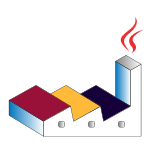
\includegraphics[width=1.65cm,height=1.05cm,keepaspectratio]{img/logo_plantuml.png} & PlantUML &
A tool that renders UML diagrams from a plain-text description. It was chosen so that the diagrams
of this report are versioned as source next to the code: a diagram that is a text file is reviewed,
diffed and corrected like anything else, whereas an exported image quietly goes out of date. \\
\hline
\centering
\includegraphics[width=1.65cm,height=1.05cm,keepaspectratio]{img/logo_lucidchart.png} & Lucidchart &
A diagramming application used for the global class diagram of Figure~\ref{fig:class-global}. That
one diagram is the map of the whole domain and needed to be laid out by hand, grouping the classes
as a reader thinks about them rather than as an automatic layout engine places them, which is what
a direct-manipulation editor does better than a text-driven one. \\
\hline
\caption{Development and modelling tools}
\label{tab:tech-tooling}
\end{longtable}

Containerization arrived later, in Sprint~10, and is presented there
(Section~\ref{sec:sprint10}) rather than here, because it was a decision the project revisited
rather than one taken at the outset.

\section*{Conclusion}
The architecture retained, a three-tier modular monolith with dynamic authorization, a hybrid
indicator engine and a normalised time-series schema, answers the requirements of Chapter~2
while remaining proportionate to the scale of the target deployment. These decisions are now
applied: the following chapters present the progressive construction of the platform, release by
release and sprint by sprint.
